%%%%%%%%%%%%%%%%%%%%%%%%%%%%%%%%%%%%%%%%%%%%%%%%%%%%%%%%%%%%%%%%%%%%%%%%%%%%%%%
%     STYLE POUR LES RAPPORTS DE PROJET
%                   NE PAS MODIFIER
%%%%%%%%%%%%%%%%%%%%%%%%%%%%%%%%%%%%%%%%%%%%%%%%%%%%%%%%%%%%%%%%%%%%%%%%%%%%%%%

\documentclass[a4paper,11pt]{article}
\usepackage[utf8]{inputenc}
\usepackage{graphicx}
\usepackage[T1]{fontenc}
\usepackage[latin1]{inputenc}
\usepackage[french]{babel}
\usepackage{float}
\usepackage{wrapfig}
\usepackage{lmodern}
\usepackage{fancyhdr}
\usepackage[top=2cm, bottom=2.7cm,right=1.5cm]{geometry}
\usepackage{tabularx}
\usepackage{array}
\usepackage{longtable}
\usepackage{hyperref}
\usepackage[final]{pdfpages} 
%%%%%%%%%%%%%%%%%%%%%%%%%%%%%%%%%%%%%%%%%%%%%%%%%%%%%%%%%%%%%%%%%%%%%%%%%%%%%%%
\usepackage{listings}
\lstset{language=xml,frame=single, breaklines=true, basicstyle=\ttfamily,backgroundcolor=\color{white},basicstyle=\scriptsize, keywordstyle=\color{blue}, commentstyle=\color{vert}, stringstyle=\color{red}, identifierstyle=\color{blue}}
\lstset{
language=Java,
basicstyle=\normalsize, % ou ça==> basicstyle=\scriptsize,
upquote=true,
aboveskip={1.5\baselineskip},
columns=fullflexible,
showstringspaces=false,
extendedchars=true,
breaklines=true,
showtabs=false,
showspaces=false,
showstringspaces=false,
identifierstyle=\ttfamily,
keywordstyle=\color[rgb]{0,0,1},
commentstyle=\color[rgb]{0.133,0.545,0.133},
stringstyle=\color[rgb]{0.627,0.126,0.941},
}

\makeatletter
\def\clap#1{\hbox to 0pt{\hss #1\hss}}%
\def\ligne#1{%
\hbox to \hsize{%
\vbox{\centering #1}}}%
\def\haut#1#2#3{%
\hbox to \hsize{%
\rlap{\vtop{\raggedright #1}}%
\hss
\clap{\vtop{\centering #2}}%
\hss
\llap{\vtop{\raggedleft #3}}}}%
\def\bas#1#2#3{%
\hbox to \hsize{%
\rlap{\vbox{\raggedright #1}}%
\hss
\clap{\vbox{\centering #2}}%
\hss
\llap{\vbox{\raggedleft #3}}}}%
\def\maketitle{%
\thispagestyle{empty}\vbox to \vsize{%
\haut{}{\@blurb}{}
\vfill
\vspace{1cm}
\par
\hrule height 4pt
\par
\begin{flushleft}
\usefont{OT1}{ptm}{m}{n}
\huge \@title
\end{flushleft}
\par
\hrule height 4pt
\par
\begin{flushright}
\usefont{OT1}{phv}{m}{n}
\Large \@author
\par
\end{flushright}

\vspace{1cm}
\vfill
\vfill
\bas{}{\@location le \@date}{}
}%
\cleardoublepage
}
\def\date#1{\def\@date{#1}}
\def\author#1{\def\@author{#1}}
\def\title#1{\def\@title{#1}}
\def\location#1{\def\@location{#1}}
\def\blurb#1{\def\@blurb{#1}}
\date{\today}
\author{}
\title{}
\makeatother
\title { \textbf{Projet Génie Logiciel - Version 1}\\
Mini-éditeur de texte} 
\author{
        Adeline \textsc{GRANET},\\
        Alexis \textsc{LINARD} \\
 }

\blurb{%
Université de Nantes\\
Master 1 ATAL\\[1em]
  
}%


 
%%%%%%%%%%%%%%%%%%%%%%%%%%%%%%%%%%%%%%%%%%%%%%%%%%%%%%%%%%%%%%%%%%%%%%%%%%%%%%%

\begin{document}          


\pagestyle{fancy}
\renewcommand{\headrulewidth}{1pt}
\renewcommand{\footrulewidth}{0pt}
\renewcommand{\headsep}{50pt}
\lhead{Mini-éditeur de texte}
\cfoot{}
\rfoot{\thepage}



\maketitle                 % Genere le titre
\thispagestyle{empty}      % Supprime le numero de page sur la 1re page

\newpage
\tableofcontents

\newpage

\section{Introduction}
\paragraph{}
Le projet \textit{Mini Editeur} a pour but la réalisation d'un outil d'éditeur de texte. Il s'inscrit dans le module de Génie Loiciel. A travers lui, nous apprenons à utiliser différents outils tel que le langage Scala avec sa bibliothèque graphique Swing dans le logiciel Éclipse ce qui nous permet de compiler, déboguer et utiliser githup pour la gestion de version. 
\paragraph{}
L’objectif de ce rapport est de présenter la modélisation de notre mini-éditeur de texte tel que nous l'avons conçu tout en intégrant les principaux diagrammes d’UML,  certains patrons de conception et ainsi que les techniques liés à l'environnement de travail.
Dans une première partie, nous présenterons le projet. L'éditeur sera présenté de manière approfondi avec ses fonctionnalités.
\paragraph{}
Dans une seconde partie, nous exposerons la vision du projet sous forme de diagramme de classe avec l'explication des patrons de conceptions utilisés. 



\section{Présentation du projet : le Mini-Editeur}
Nous allons présenter dans cette partie l'éditeur de texte dans sa globalité avec les différentes fonctionnalités que l'on devra intégrer ainsi que le contenu de chaque version.

\subsection{Le principe}
Ce projet reste un éditeur de texte tout ce qu'il y a de plus basique avec les fonctionnalités qu'on lui connait. Certains conceptions et fonctionnalités nous ont été imposé comme suit : 
\begin{itemize}
\item le texte est contenu dans un Buffer (zone de travail);
\item il existe une notion de sélection de texte, avec des commandes utilisateur permettant de déplacer le début et la fin de la sélection; 
\item copie de la sélection dans le presse-papier; 
\item copie de la sélection dans le presse-papier puis effacement de la sélection;
\item remplacement de la sélection par le contenu du presse-papier;
\item l'interface homme-machine est d'un type quelconque (textuelle ou graphique).
\end{itemize}
Pour ce dernier point, nous avons choisi une version graphique simple pour interagir avec l'utilisateur.

\subsection{En plusieurs versions}
La conception du logiciel doit se faire en spirale c'est-à-dire fournir des livrables à intervalle donné et enrichir la version précédente à chaque fois. Nous aurons trois version de l'éditeur de texte. 
\begin{description}
\item la version 1 contiendra uniquement les actions d'édition de base ainsi que l'interface graphique correspondante;
\item la version 2 permettra d'enregistrer les actions de l'utilisateur et de les rejouer;
\item la version 3 permettra de réaliser le défaire/refaire, avec une capacité quelconque dans le défaire (c'est-à-dire être capable de revenir à l'état initial)
\end{description}
A chaque étape, nous ferons évoluer l'interface graphique en conséquence de l'ajout/modification des différentes options.

\paragraph{}
Ce projet est conçu pour que l'on puisse répondre à certains objectifs pédagogique qui ont été fixé comme être capable de présenter une tehnique de conception en utilisant différents patrons de conception; être capable de faire en parallèle la réalisation de diagramme statique et dynamique en UML.

\paragraph{}
Dans ce rapport c'est donc la première version que nous allons présenter avec le(s) patron(s) mis en jeu.

\section{Implémentation de la version 1}


\begin{figure}[!ht]
		\center
		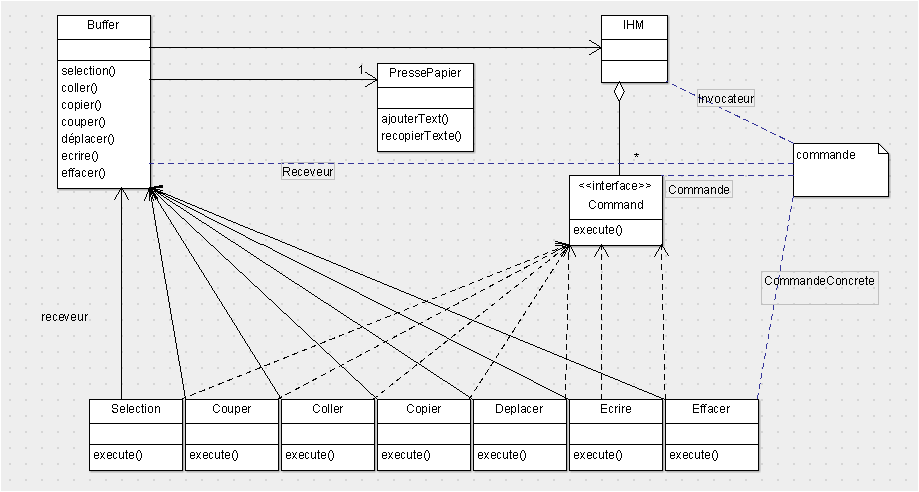
\includegraphics [width=15cm]{Command.png}
		\caption{Mise en oeuvre du patron Commande}
\end{figure}

\section{Conclusion}


\newpage
\listoffigures  % table des figures
\listoftables
\newpage
\nocite{*}
\bibliographystyle{unsrt} % Le style est mis entre accolades.
\bibliography{biblio} % mon fichier de base de données s'appelle bibli.bib
\newpage



\end{document}
